\chapter{Debugging support}

\begin{quote}
  \textit{Debugging is twice as hard as writing the code in the first place.
    Therefore, if you write the code as cleverly as possible, you are, by
    definition, not smart enough to debug it.}\begin{flushright}
    \tiny{Brian W. Kernighan}
  \end{flushright}
\end{quote}

We already mentioned in the first chapter that to debug programs written in
high level programming languages, we need the compiler to emit debugging
information. But debugging support must also be provided by operating system
(if there is one) and by processor itself. However, we can still debug programs
in machine code. We briefly mentioned this in chapter 1 \todo{ref}, however, we
won't see source code, but only assembly. This can still be useful, for example
for reverse engineering. And, as was already hinted, source level debugging is
built upon assembly debugging. In this chapter, we will describe on which
levels must assembly level debugging be supported. Additionaly, we'll discuss
how are compilers and debuggers able to allows us to debug source code
althrough the programs are still machine code programs. 

\section{Support on CPU level} In first chapter it was said that CPU can only
execute machine code which is made of instructions and that it has certain
registers. Which instructions and registers the CPU has can differ from CPU to
CPU. This is specified by \textit{Instruction Set Architecture} (ISA)
\cite{aps-isa}. It is an abstract interface between the hardware and lowest
level software (machine code). It contains all information needed to write a
program in machine code. In general, ISA specifies following: 
\begin{itemize}
    \item Set of machine code instructions - Specifies instructions the ISA has
          and what operands each instruction has.
    \item Register set - Which
          registers the ISA has\footnote{Strictly speaking ISA doesn't have
          to use registers. It's possible to use only stack or accumulator,
          but most used ISAs use registers, so we'll ignore those
          architectures. }.   
    \item Addressing modes - Possible methods to refer to memory or register. 
\end{itemize} There are other specification,
however they are not relevant to this thesis. For each instruction and operand
there is specified how they should be encoded into binary (remember, that's
what the CPU can understand). CPU then \textit{implements} some ISA. If two
different CPUs implements the same ISA then they should be able to run the same
machine code program. For example, most PC use the \textit{x86} architecture
\cite{aps-isa}, althrough the ARM architecture is also seeing use in personal
computers, for example the Apple Sillicon is of ARM architecture.

The x86 architecture is so called \textit{Complex Instruction Set Architecture}
(CISC). It contains many instructions that do many things at once, have varying
length and takes multiple clock cycles to complete \cite{intel-manual}. On the
other hand the ARM architecture is \textit{Reduced Instruction Set
Architecture} (RISC). The number of instructions is smaller, they are intended
to be small building blocks from which complex operations may be created by
using many of them. Each instruction in RISC also has same length. Both
architectures have their pros and cons, althrough some literature suggest that
in modern days the choice of architecture is irrelevant if one is only
considering performance and power
consuption  \cite{riscvscisc1, riscvscisc2}. Unless specified otherwise the
rest of this chapter will be talking about x86. This is because T86 \todo{ref}
is loosely based on x86, so it is most relevant for us.

In first chapter we briefly mentioned that machine code programs can instead be
written in Assembly language. Assembly is almost 1:1 mapping to machine code.
When showing programs, we will show them in assembly. In figure
\ref{fig:assembly-example2}, we present another example of a program that was
compiled from C to assembly of the x86 architecture. As seen, instructions have
various operands. Most often registers (\texttt{RBP, RSP, EAX}), memory
(\texttt{[rbp-4]} is reference to memory at address which is in register
\texttt{rbp} minus $4$), or labels (like \texttt{L2}). Labels are not part of
machine code, instead memory address has to be provided. This is a small part
where assembly and machine code differ. For detailed overview of the x86
instructions see \cite{intel-manual}.

\begin{figure}\label{fig:assembly-example2}
    \begin{lstlisting}
max:
    push    rbp
    mov     rbp, rsp
    mov     QWORD PTR [rbp-24], rdi
    mov     DWORD PTR [rbp-28], esi
    mov     rax, QWORD PTR [rbp-24]
    mov     eax, DWORD PTR [rax]
    mov     DWORD PTR [rbp-4], eax
    mov     DWORD PTR [rbp-8], 1
    jmp     .L2
.L3:
    mov     eax, DWORD PTR [rbp-8]
    cdqe
    lea     rdx, [0+rax*4]
    mov     rax, QWORD PTR [rbp-24]
    add     rax, rdx
    mov     eax, DWORD PTR [rax]
    cmp     DWORD PTR [rbp-4], eax
    cmovge  eax, DWORD PTR [rbp-4]
    mov     DWORD PTR [rbp-4], eax
    add     DWORD PTR [rbp-8], 1
.L2:
    mov     eax, DWORD PTR [rbp-8]
    cmp     eax, DWORD PTR [rbp-28]
    jl      .L3
    mov     eax, DWORD PTR [rbp-4]
    pop     rbp
    ret
    \end{lstlisting}
    \caption{Compiled C program with GCC 9.4 compiler as x86 assembly.}
\end{figure}

\subsection{Registers}

The x86 architecture has a set of general purpose registers.
Some of these are
\begin{itemize}
    \item RAX - Accumulator for operands and results data,
    \item RCX - Counter for string and loop operations,
    \item RSP - Stack pointer,
    \item RBP - Pointer to data on the stack.
\end{itemize}
The names and number of general purpose registers change based on bit mode.
64-bit (also named x86-64) mode has 16 of them, while 32-bit has 8. Althrough
the \texttt{RSP} and \texttt{RBP} are called general purpose they are often
only used for pointing at the top of the stack, resp. to the base of the stack.
Stack is special part of program memory, it mostly has LIFO
semantics\footnote{For example the \texttt{mov eax, DWORD PTR [rbp - 4]} does
not respect LIFO semantics, because it reads directly from the stack and not
from the top.} It can be used to store intermediate result, arguments to
functions, return address etc. This register is weird in a sense that it has
this very special purpose but is still considered part of the general purpose
registers~\cite{intel-manual}. One might use it for storing calculations, but
it would make rest of the instructions that work with stack behave
unexpectedly.

Instruction pointer register (RIP on x86-64, EIP on x86) contains address of
the current instruction to be executed. As we mentioned in Introduction
\todo{ref}, programs are executed sequentially from top to bottom, with certain
instructions having the ability to change the control flow. When an instruction
get executed, the size of the instruction will be added to the value in RIP
register. This will advance the instruction pointer to the next instruction.
Or, if the instruction changes control flow, the value in instruction pointer
will be changed to the destination of the instruction. The register can also be
changed directly.

Another interesting register is the \texttt{EFLAGS} register. The register
contains group of flags, which can alter various behavior of the CPU, or the
CPU itself sets them as result of some instruction. For example the instruction
\texttt{cmp} compares its two operands and if they are the same the
\textit{zero} flag in the \texttt{EFLAGS} register will be set.

\subsection{Interrupts}
Interrupt is a special request to the CPU to stop execution of current program
and to quickly react to the reason that caused the request
\cite{aps-interrupts}. Example of such event can be keyboard press or error in
an program (division by zero). There are two main categories
\cite{intel-manual}
\begin{itemize}
    \item An \textbf{interrupt} is an asynchronous\footnote{Meaning that the
    interrupt may happen when another instruction is being processed (not on
the CPU clock edge).} event that is typically triggered by an Input/Output (IO)
device. \item An \textbf{exception}\footnote{Unfortunately, this term will
    become quite overloaded in this thesis.} is a synchronous event that is
        generated when the processor detects one or more predefined conditions
        when executing an instruction. These are further divided into three
        classes: faults, traps and aborts.
\end{itemize}

When an interrupt or exception happens, the processor halts execution of
current program and switches to specific interrupt handler. Interrupt handler
is just another sequence of instructions that handles the interrupt. Example of
an exception is the \texttt{INT3} instruction. When this instruction is
executed an interrupt is generated. This instruction is specifically meant to
be used as a breakpoint. We can supply code that will be responsible for
handling the breakpoint as the interrupt handler. However, on modern PCs a
Operating System (OS) is governing the PC. Alas, we cannot touch the interrupt
handler directly. Instead, an OS is going to have to provide another layer of
support for debugging.

Recall the EFLAGS register mentioned in section \ref{X}. There is a special
flag called trap flag. When it is set, cpu will issue an interrupt after every
executed instruction. This could be useful if we wanted to inspect execution
instruction by instruction.

\todo{Debugging embedded and hardware breakpoints}

\section{Operating system support} Operating system is a layer between computer
components (cpu, memory, input/output devices, \dots) and software. It is
responsible for handling all those resources so programmers do not have to
think about it \cite{modern-os, os-concepts}. Managing resources is not only to
make writing programs easier, but to make sure that they are safe from each
other. Modern operating system allows to run multiple programs at once (or at
least offer the illusion that it can) and they make sure that one program
cannot overwrite data or otherwise interfere with other programs. Normal
programs runs in so called \textit{user space}, which has limited capabilites.
Kernel on the other hand runs in \textit{kernel space}. It has full access to
hardware of the computer, can use all instructions, can permit or mask
interrupts and so on.

However, if programs were limited to user space all the time they would be very
limited. Sometimes, they need to escape the confiment of the OS, for example to
read a file or communicate with other processes. Operating systems provide an
interface through which the user space program can leverage small part of the
kernel - system calls. They offer a way of requiring some service from the OS.
This API is often in form of C and C++ functions~\cite{os-concepts}. A part of
these functions is a special instruction, like \texttt{SYSCALL} on
x86~\cite{intel-manual}, that switches the mode to kernel space. The kernel has
to check if the call is correct, since it will be executed in kernel space with
full access.

The most prelevant operating systems today are Microsoft Windows, Linux and MacOS.
Linux and MacOS systems are somewhat similar, but Windows is very different.

\subsection{Linux}
Linux offers special system call which is very handy for debugging. It is
called \texttt{ptrace} \cite{ptrace} - process trace. It has following
signature: \texttt{ptrace(PTRACE\_COMMAND, pid, ...)}. It takes a
\texttt{PTRACE\_COMMAND}, which specifies the behaviour of the function (for
example \texttt{PTRACE\_SINGLESTEP} for single step), pid of some process and
some other parameters, depending on the \texttt{PTRACE\_COMMAND} that was
chosen. It allows to observe and control the execution of another process, this
process will be the debugee. In the context of \texttt{ptrace}, we will instead
use the word tracee for the debugee, and tracer for the debugger, to be
consistent with ptrace documentation.

\texttt{ptrace} has many commands, here are some of the most important:
\begin{itemize}
    \item \texttt{PTRACE\_PEEKTEXT, PTRACE\_PEEKDATA} - Read tracee's memory,
    \item \texttt{PTRACE\_POKETEXT, PTRACE\_POKEDATA} - Write into tracee's memory,
    \item \texttt{PTRACE\_GETREGS} - Read tracee's register values,
    \item \texttt{PTRACE\_SETREGSET} - Modify tracee's register values,
    \item \texttt{PTRACE\_GETSIGINFO} - Retrieve information about the signal
                                        that caused tracee to stop,
    \item \texttt{PTRACE\_CONT} - Restart the stopped tracee process,
    \item \texttt{PTRACE\_SINGLESTEP} - Restart the stopped tracee but
          stop it after executing one instruction.
\end{itemize}

Linux however needs some way of notifying the debugger that the tracee
encountered a breakpoint, or that some other event requiring debugger attention
happened. To this end, \textit{signals} are used. They are in principle similar
to CPU interrupts. They are however on the OS level. A signal is used in UNIX
and Linux systems to notify a process that a particular event has occured
\cite{os-concepts}. Signals can be sent to processes. When such process
receives a signal, it stops its execution and starts the execution of a signal
handler. There are various signal types. Most signals can have custom signal
handler defined by the process. If no handler is defined then a default one is
provided by the OS. However handlers for \texttt{SIGKILL} and \texttt{SIGSTOP}
cannot be changed \cite{signals}.

Reason for rising a signal can be \todo{Tady toho asi bude vic}
\begin{itemize}
    \item CPU Interrupt (Division by zero, Breakpoint hit),
    \item System call (\textit{kill(pid, signal)}).
\end{itemize}

For example, the signal \texttt{SIGTERM} can be send to a process to ask it
nicely to exit. The process can handle this request, for example to save some
state before exiting. It can also however be completely ignored. For this, a
signal \texttt{SIGKILL} can be used, which cannot be handled, ignored or
blocked.

To begin tracing a command \texttt{PTRACE\_ATTACH} may be used for already
existing process, or a \texttt{fork} followed with child calling
\texttt{PTRACE\_TRACEME} and typically \texttt{execve}. When the tracee is
being traced it will stop each time a signal is delivered to it, even if it
choose to ignore said signal. The tracer will be notified at its next call to
the \texttt{waitpid} function. It will return a value which indicates the cause
of the stop in the tracee. When the tracee is stopped the tracer can initiate
various ptrace request listed above to inspect and change the state of the
tracee \cite{ptrace}.

In the CPU chapter we mentioned that there are debug instructions and that they
issue an interrupt. We do not directly handle the interrupt here. Even if we
wanted, user space programs can't do that. The Linux kernel handles this for us
and instead uses the signals as an abstraction. \todo{Include kernel code.}

\subsubsection{Debugger implementation}
Now, we have all the necessary building blocks to build a simple debugger on
the Linux operating system running on the x86 platform. Running a program under
the debugger is simple. On figure \ref{fig:debugger-init} you can see the
initialization of the debugger. It uses the fork-exec idiom. \texttt{fork}
system call creates an exact copy of the process as a child except the
following: process ID (PID) of the child is different. In the parent process,
PID of the child is returned, in the child a $0$ is returned. In the child, we
initiate the \texttt{PTRACE\_TRACEME} call, which indicates that this process
is to be traced by its parent. Then it calls \texttt{execve} system call, which
replaces this program with the one we want to debug. The execve causes a
\texttt{SIGTRAP} signal on completetion because it is being traced
\cite{execve}.

The parent first issues a \texttt{waitpid} system call. This waits for the
childs \texttt{execve} to finish. The debugger then has a chance to debug the
child immediately, because it is stopped. The \texttt{while} loop can then
request input from user and act accordingly. The tracee can be continued by
\texttt{PTRACE\_CONT} command.

\begin{figure}\label{fig:debugger-init}
    \begin{minted}{c}
        pid_t pid = fork();
        if (pid == 0) {
            // Begin tracing
            ptrace(PTRACE_TRACEME, 0, NULL, NULL);
            // Replace the code with the intended tracee code
            execve(executable, argv, NULL);
        } else {
            int w;
            waitpid(pid, &w, 0);
            while(...) {
                // Main debugger loop
            }
        }
    \end{minted}
    \caption{Linux - Debugger initialization.}
\end{figure}

Rest of the examples will be taken from the \textit{LLDB} debugger
\todo{Perhaps link the concrete file where are those functions located?}. They
will be abbreviated and sometimes some code will be cut (like error handling)
to demostrate the example more clearly and to show that real world debuggers
actually do use those techniques. LLDB has all ptrace calls wrapped in another
function which handles errors and if the signal was interrupted by other
signal. This function is called \textit{PtraceWrapper}.

Reading and writing to memory is simple. The \texttt{PTRACE\_PEEKTEXT} and
\texttt{PTRACE\_POKETEXT} are used for this purpose. This call reads or writes
a word (32 or 64 bits, depending on the Linux variant) into tracees memory.
However, if we want to write arbitrary amount of bytes, we have to work around
the word limitation. We need to write by blocks and for the last one we have to
pad the write with already existing data if the block size does not divide the
word size. In figure \ref{fig:write-read} is shown how to read and write
exactly one byte of memory at given address.

\begin{figure}\label{fig:write-read}
    \begin{minted}{c}
uint8_t read_memory(pid_t pid, uint64_t address) {
    uint64_t data = ptrace(PTRACE_PEEKDATA, pid, address, NULL);
    return (uint8_t)data;
}

void write_memory(pid_t pid, uint64_t address, uint8_t data) {
    uint64_t old_data = ptrace(PTRACE_PEEKDATA, pid, address, NULL);
    uint64_t new_data = (old_data & ~0xFF) | data;
    ptrace(PTRACE_POKEDATA, pid, address, new_data);
}
    \end{minted}
    \caption{Linux - Reading and writing one byte using ptrace.}
\end{figure}

Registers are similar to memory in regards how to read them. Linux contains
predefined structure \texttt{user\_regs\_struct}, which maps all registers on
current architecture. The command \texttt{PTRACE\_GETREGS} then fills up this
structure with the value in registers. To save registers,
\texttt{PTRACE\_SETREGS} can be used. One has to pass the whole structure, so
if we want to modify only some registers we first need to fetch the structure,
fill the registers we want with values, and then finally use \texttt{SETREGS}.
An implementation can be seen on figure \ref{fig:set-register}, the
\texttt{get\_register} functions maps the structure members to register name.
Since the address of current instruction to be executed is also stored in
register, we now have access to it.

\begin{figure}\label{fig:set-register}
    \begin{minted}{c}
void set_register(pid_t pid, const char* name, uint64_t data) {
    struct user_regs_struct regs;
    ptrace(PTRACE_GETREGS, pid, NULL, &regs);
    uint64_t* reg_data = get_register(&regs, name);
    *reg_data = data;
    ptrace(PTRACE_SETREGS, pid, NULL, &regs);
}
    \end{minted}
    \caption{Linux - Setting one register using ptrace}
\end{figure}

Breakpoints are more interesting. Debuggers often allow to enable and disable
breakpoint, so we will distinguish setting a breakpoint and enabling it.
Setting a breakpoint just means that the debugger needs to keep track where the
breakpoint was set and if it is enabled or disabled. Enabling a breakpoint
means writing into the program memory the debug instruction (we will use the
x86 \texttt{INT3} with opcode \texttt{0xCC}). On figure
\ref{fig:with-and-without-bp} there is shown how code looks with and without
enabled breakpoint. On line $2$, the opcode changes from \texttt{0x83} to
\texttt{0xCC}. Since the breakpoint is set via the \texttt{PTRACE\_POKEDATA},
which only works data blocks, one has to pad the breakpoint opcode with already
existing data. Also, the rewriten data has to be kept so that the breakpoint
may later be deactivated. Abbreviated implementation can be found on
\ref{fig:breakpoint-enable}.

\begin{figure}\label{fig:with-and-without-bp}
    \begin{minipage}{0.45\textwidth}
        \begin{lstlisting}
c7 45 fc 05 00 00 00 	MOVL
83 7d fc 00          	CMPL
7e 07                	JLE
        \end{lstlisting}
    \end{minipage}
    \begin{minipage}{0.45\textwidth}
        \begin{lstlisting}
c7 45 fc 05 00 00 00 	MOVL
cc 7d fc 00          	INT3
7e 07                	JLE
        \end{lstlisting}
    \end{minipage}
    \caption{Code with and without breakpoint.}
\end{figure}

\begin{figure}\label{fig:breakpoint-enable}
    \begin{minted}{c}
void enable(pid_t pid, struct breakpoint* bp) {
    if (bp->enabled) {
        return;
    }
    bp->backup = read_memory(pid, bp->address);
    write_memory(pid, bp->address, BP_OPCODE);
    bp->enabled = true;
}

void disable(pid_t pid, struct breakpoint* bp) {
    if (!bp->enabled) {
        return;
    }
    write_memory(pid, bp->address, bp->backup);
    bp->enabled = false;
}
    \end{minted}
    \caption{Enabling breakpoints, abbr.}
\end{figure}

When breakpoint is hit, the control is passed to the debugger, at this point,
the instruction pointer would point to the next instruction, which has opcode
\texttt{0x7D}, not \texttt{7E} (the \texttt{JLE} instruction) as might be
expected. This is because \texttt{INT3} is instruction with size $1$. It gets
executed, instruction pointer is advanced by the size ($1$) and interrupt is
issued. But after the INT3 there were operands to the CMPL instruction, we
definitely do not want to interpret them as instruction. On some architectures,
advancing PC does not happen for the debug instruction (like ARM \todo{Checked
by hand - Reverse engineered from LLDB source code}.).

Additionaly, if we just moved back and resumed the program, we would again hit
the breakpoint which is still set! We need to temporarily unset it, move one
instruction forward, and set it again. The general idea behind it can be found
on figure \ref{fig:continue}. With breakpoints, we essentially gained the
ability to single step as well. 

\begin{figure}\label{fig:continue}
    \centering
    \includegraphics[width=100mm,scale=0.5]{media/breakpoint_tbd}
    \caption{Continue sketch}
\end{figure}

We showed that the breakpoint must be put
at the next instruction. This is not as simple as it sounds. Where is next
instruction? On CISC architectures, this is not easy to find out since
instructions have different sizes. But even on RISC architectures like ARM,
what if the instruction is a jump of some sort and the next instruction is not
simply the one that follows this one in the code? For this reason, debuggers may
need to have an instruction emulator, which needs to emulate whole instruction
set to see where the program counter ends up\footnote{And there can be a
\textit{lot} of instructions \cite{intel-manual}}. However, some architectures
offer hardware support, like the trap flag we mentioned in section \todo{ref}.

The ptrace library contains special \texttt{PTRACE\_SINGLESTEP} command. This
executes one instruction in the tracee and then signal \texttt{SIGTRAP} will be
sent to it. The linux kernel (as of v6.1.8) uses previously mentioned trap flag
for x86 \cite{linuxkernel-trapflag}. If the architecture does not provide a way
to support single stepping then the call will return an error. If we are on an
architecture that support this command we can use it instead of the register
dance mentioned above. Implementation is described on figure
\ref{fig:singlestep}. We presume that the instruction pointer was moved when
the breakpoint was hit, so we do not need to return one byte backward. This is
more reasonable anyway, since you want to show the user at which address was
the breakpoint hit.

\begin{figure}\label{fig:singlestep}
    \begin{minted}{c}
void step_over_bp(pid_t pid) {
    uint64_t loc = read_register(pid, "rip");
    struct breakpoint* bp = find_bp(loc);
    if (bp == NULL || !bp->enabled) {
        return;
    }

    disable(pid, bp);
    ptrace(PTRACE_SINGLESTEP, pid, NULL, NULL);
    // Waits until debugee finishes singlestepping
    wait_for_debugee(pid);
    enable(pid, bp);
}
    \end{minted}
    \caption{Stepping over breakpoint, abbreviated.}
\end{figure}

For normal single step, we can just use the \texttt{PTRACE\_SINGLESTEP} command.
We however need to check if the current line doesn't have a breakpoint, since
that would cause or debugger to return the program counter back before it and
we wouldn't be able to step over it. So, if there is a breakpoint use the code
from \texttt{fig:singlestep}, else just use \texttt{PTRACE\_SINGLESTEP}.

Step over is more entertaining. It is used to jump out of current function.
When a procedure is entered using the \texttt{call} instruction, the address
immediately after the call instruction is put onto the stack. Then, on entry to
the function \texttt{rbp} register is pushed onto the stack and then the value
of it is set to the current value of stack pointer. So the return address is
located at \texttt{rbp + 8}. We can set breakpoint at that address and then
continue execution, wait for the debugee to hit the breakpoint and then disable
and remove it. This has its flaws, for example it won't work if the step out is
used before the rbp is set. Or if some library completely bypasses the call
instruction.

\subsection{Windows}
\todo{WIP: Will be rewritten (probably shortened)}
Windows also has built-in support for debugging at the Win32API layer
\cite{windows-msdn-debugging-api, windows-press-debugging-api}.
It builds on \textit{debug events} and \textit{debug functions}. Summary of
some of the functions that Win32 API offers which all help with debugging:

\begin{itemize}
    \item \mintinline{c}{DebugActiveProcess} - Attaches the debugger to an active process.
    \item \mintinline{c}{DebugBreakProcess} - Causes a breakpoint exception to occur in the specified process.
                                          This passes control of the process to the debugger if there is one.
    \item \mintinline{c}{WaitForDebugEvent} - Waits for new debug events.
    \item \mintinline{c}{ContinueDebugEvent} - Continue the process execution after processing debug event.
    \item \mintinline{c}{OutputDebugString} - Sends a string to the debugger for display.
    \item \mintinline{c}{ReadProcessMemory} and \mintinline{c}{WriteProcessMemory} - Read and modify
          process virtual address space.
    \item \mintinline{c}{FlushInstructionCache} - Flushes instruction cache of the process.
\end{itemize}

The general structure of Windows debugger can be seen in figure \ref{fig:win32debugger}.
The debugger waits for debug events via function \mintinline{c}{WaitForDebugEvent}.
This function has a timeout parameter, so the debugger can also do other things while it's waiting.
These events are put in a queue, so the debugger will not miss any.

\begin{figure}
    \centering
    \scalebox{0.8}{
    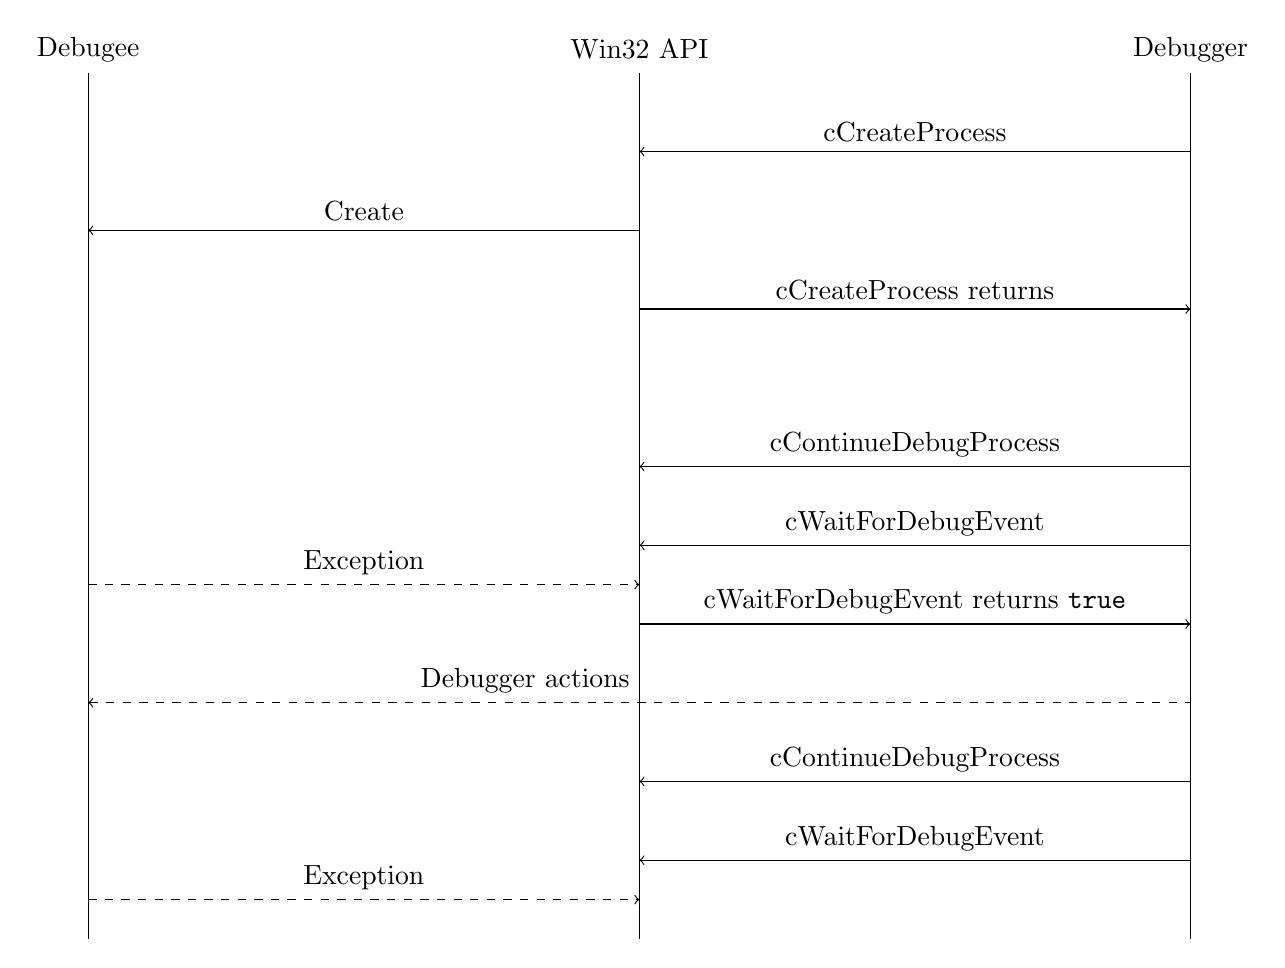
\begin{tikzpicture}
        \draw (-7,0) -- (-7,-11) (0,0) -- (0,-11) (7,0) -- (7,-11);
        \node at (-7,.3) {Debugee};
        \node at (0,.3) {Win32 API};
        \node at (7,.3) {Debugger};
        \draw[<-] (0,-1) -- node[midway,above] {\mintinline{c}{CreateProcess}} (7,-1);
        \draw[<-] (-7,-2) -- node[midway,above] {Create} (0,-2);
        \draw[->] (0,-3) -- node[midway,above] {\mintinline{c}{CreateProcess} returns} (7,-3);
        \draw[<-] (0,-5) -- node[midway,above] {\mintinline{c}{ContinueDebugProcess}} (7,-5);
        \draw[<-] (0,-6) -- node[midway,above] {\mintinline{c}{WaitForDebugEvent}} (7,-6);
        \draw[dashed,->] (-7,-6.5) -- node[midway,above] {Exception} (0,-6.5);
        \draw[->] (0,-7) -- node[midway,above] {\mintinline{c}{WaitForDebugEvent} returns \texttt{true}} (7,-7);
        \draw[dashed, <-] (-7, -8) -- node[above left] {Debugger actions} (7, -8);
        \draw[<-] (0,-9) -- node[midway,above] {\mintinline{c}{ContinueDebugProcess}} (7,-9);
        \draw[<-] (0,-10) -- node[midway,above] {\mintinline{c}{WaitForDebugEvent}} (7,-10);
        \draw[dashed,->] (-7,-10.5) -- node[midway,above] {Exception} (0,-10.5);
    \end{tikzpicture}
    }
    \caption{A sequence diagram for debugger using Windows api. Inspired by \todo{NI-REV 6. lecture}}
    \label{fig:win32debugger}
\end{figure}

The debug events are thoroughly described in subsection \ref{section:Debug Events}. The main point of interest is the exceptions.
By these, we do not mean the standard C++ exceptions but rather Microsoft \textit{Structured Exception Handling}.

\subsubsection*{Debug Events}\label{section:Debug Events}
Debugging events are various incidents in the debuggee that causes the system
to notify the debugger \cite{windows-msdn-debug-events}. These are stored in
special \mintinline{c}{DEBUG_EVENT} structure, which is received in
\texttt{WaitForDebugEvent} call from debugger. This structure contains various
information about the event, the internals can be seen on figure
\ref{fig:DebugEvent}. These events include loading and unloading a DLL,
creating and exiting a process, sending debug strings via the
\mintinline{c}{OutputDebugString} and so on. It also includes exceptions, those
are probably the most important for us. 

\begin{figure}
\begin{minted}{c}
typedef struct _DEBUG_EVENT {
  DWORD dwDebugEventCode;
  DWORD dwProcessId;
  DWORD dwThreadId;
  union {
    EXCEPTION_DEBUG_INFO      Exception;
    CREATE_THREAD_DEBUG_INFO  CreateThread;
    CREATE_PROCESS_DEBUG_INFO CreateProcessInfo;
    EXIT_THREAD_DEBUG_INFO    ExitThread;
    EXIT_PROCESS_DEBUG_INFO   ExitProcess;
    LOAD_DLL_DEBUG_INFO       LoadDll;
    UNLOAD_DLL_DEBUG_INFO     UnloadDll;
    OUTPUT_DEBUG_STRING_INFO  DebugString;
    RIP_INFO                  RipInfo;
  } u;
} DEBUG_EVENT, *LPDEBUG_EVENT;
\end{minted}
\caption{Structure which contains info about debug event.}
\label{fig:DebugEvent}
\end{figure}

\subsubsection*{Structured Exception Handling}
This feature is specific to Windows only. For example, if division by zero was
performed in a program on Linux, a signal would be sent to the process. Windows
don't have signals, instead, it uses Structured Exception Handling
\cite{windows-msdn-seh}. From now on, we will be using the abbreviation 'SEH'.
An exception is an event that requires execution of code outside the normal
flow of control. There are software exceptions, like throwing an exception
explicitly or by OS, and hardware exceptions, like the division by zero we
mentioned. Instruction with opcode \mintinline{c}{0xCC}, which is used for
breakpoints, will also raise an exception. SEH unifies both of these things
into one.

When an exception is triggered, control is transferred to the system. It saves
the state of the thread and some other information. This information can be
used to continue execution from the point where the exception was thrown when
it is resolved. It also contains information about which type of exception was
thrown, if execution can continue after handling the exception, address where
the exception occured and some others\footnote{See MSDN documentation
\cite{windows-msdn-seh} for full detailed list}. The system then searches for
an exception handler which will handle the exception. The search is performed
in this order:

\begin{enumerate}
    \item If the process is debugged the debugger is notified.
    \item If it is not or the debugger does not handle the exception, the frame-based exception handler is to be found\footnote{The handlers are not very important to us, see MSDN documentation if you're interested \cite{windows-msdn-seh}.}
    \item If no frame-based handler can be found, or no handler handles the exception, but the process is being debugged then the debugger gets notified once again.
    \item The system provides default handling, which is to terminate the program via \mintinline{c}{ExitProcess} most of the time.
\end{enumerate}

Here we see that every exception that occurs in the debuggee causes the
debugger to be notified. Breakpoints are also caused by an exception, as was
briefly mentioned before. There are two possible notifications to the debugger.
The first is known as \textit{first-chance} notification
\cite{windows-msdn-dbg-exc-handling}. The debugger can (and should) inspect the
information about the exception and see if it was a breakpoint or single-step.
These only occurs if the process is debugged (it wouldn't happen otherwise) and
the debugger should handle them. If it is something else it can ignore the
exceptions. When the program is continued via
\mintinline{c}{ContinueDebugEvent}\footnote{This function has a special
parameter, which is used to tell that the exception was or was not handled.},
the debugger is notified once again if no appropriate exception handler was
found for the exception. This is known as \textit{last-chance} notification
because if the debugger does not handle the exception the debuggee will be
terminated. It gives the user a chance to debug why is his process terminating.

Here are some exceptions that tie into debugging:
\begin{itemize}
    \item \mintinline{c}{STATUS_BREAKPOINT} - Raised when a hardware-defined breakpoint was encountered. This includes the mentioned \mintinline{c}{INT3} instruction.
    \item \mintinline{c}{STATUS_SINGLE_STEP} - Raised when a single step was completed, ie. when instruction was executed and the trap flag is set.
\end{itemize}

\subsubsection*{Tying it all together}
Now we have all necessary building block to build a simple proof of concept
Windows debugger. On figure \ref{fig:windows-debugger-mainloop}, you can see a
basic idea of a main loop of the debugger. It waits for debug events and
branches depending of the type of event. It needs not only handle exceptions,
but other events also. For example if the debugee creates a thread that is
something the debugger should be aware of. Modern debuggers trace all threads
of the program.

\todo{Pridat dalsi figure kde je jak se hanndlujou tyhle blbosti} However,
exceptions are the most interesting for us. There, breakpoint and single step
handling should be done. On both of these, the debugger should handle the
exception itself, so this is the \textit{first chance} notifications. There is
also an \mintinline{DBG_CONTROL_C}, which happens on CTRL + C keyboard press.
This should terminate the program. The debugger will pass the first chance and
catch the last chance exception, so user has a final chance to look at the
program state before it exits.

\begin{figure}
    \begin{minted}{c}
void EnterDebugLoop(const LPDEBUG_EVENT DebugEv)
{
   DWORD dwContinueStatus = DBG_CONTINUE; // exception continuation
   for(;;)
   {
      WaitForDebugEvent(DebugEv, INFINITE);
      switch (DebugEv->dwDebugEventCode)
      {
         case EXCEPTION_DEBUG_EVENT:
            // Handle exception debug events
         // Other debug events
      }
   ContinueDebugEvent(DebugEv->dwProcessId,
                      DebugEv->dwThreadId,
                      dwContinueStatus);
   }
}
\end{minted}
\caption{Windows debugger main loop}
\label{fig:windows-debugger-mainloop}
\end{figure}

\section{Compiler support}
\todo{WIP: Moved from introduction here for the time being}
When we talked about evolution of programming from machine code to assembly to
higher level languages, we haven't talked about how they are executed. Machine
code can be directly executed by processor, as we said, it is a sequence of
binary. Assembly is text, processors don't understand text. But assembly can be
mapped to machine code almost 1:1\footnote{There are some exceptions, like
labels. But translating them is not very difficult.}.

However, high level programming languages do not map 1:1 to assembly. Some are
close to it, like C, while others are miles away, like Haskell. But as was
said, processors understand only machine code. To this end, programs that can
translate source code into machine code, were created. They are called
compilers and the translation process is called compiling. For example, for the
C language one might use the GCC or Clang compilers. On figure
\ref{fig:compiler-structure} can be seen basic structure of a compiler
\cite{dragon-book}. 

\tikzstyle{compilerblock} = [rectangle, draw, minimum width=6cm, minimum height=1cm] 
\tikzstyle{tables} = [rectangle, draw, minimum width=4cm, minimum height=1cm] 
\begin{figure}\label{fig:compiler-structure}
    {\centering
    \begin{tikzpicture}
    \node (lexer)[compilerblock]{Lexical analyzer};
    \node (syntax)[compilerblock,below=of lexer]{Syntactic analyzer};
    \node (semantic)[compilerblock,below=of syntax]{Semantic analyzer};
    \node (imc)[compilerblock,below=of semantic]{Intermediate Code Generator};
    \node (gen)[compilerblock,below=of imc]{Code Generator};
    \node (symbol)[tables, left=of semantic]{Symbol table};
    \draw[->] (lexer) -- node[below] {} (syntax);
    \draw[->] (syntax) -- node[below] {} (semantic);
    \draw[->] (semantic) -- node[below] {} (imc);
    \draw[->] (imc) -- node[below] {} (gen);
    \end{tikzpicture} 
    \par}
    \caption{Simplified structure of a compiler. Some parts were left out, like optimizations.}
    \label{fig:compiler_tikz}
\end{figure}

\subsection{Lexical analyzer}
The lexical analyzer groups separate symbols into groups. For example the code
\begin{minted}{c}
foo = bar(1 + 2);
\end{minted}
might be translated into tokens like this
\begin{lstlisting}[stringstyle=\color{black}]
<id:"foo"> <assignment-operator> <id:"bar"> 
<left-bracket> <int-number:1> <plus-operator> 
<int-number:2> <right-bracket> <semicolon>
\end{lstlisting}
The Syntactic analyzer then works with these tokens.

\subsection{Syntantic and semantic analyzer}
Syntactic analysis accepts tokens and processes them into other intermediate
representation. This is most often an abstract syntax tree (abbr. AST, figure
\ref{fig:ast}). It also checks that the source code complies to the grammar of
the language. Semantic analysis then checks that the program is semantically
consistent. For example that used variable has been declared before.

\begin{figure}\label{fig:ast}
    \centering
    \begin{tikzpicture}[,shorten >=1pt,node distance=1.8cm,on grid,initial/.style={}]
    \node (assignment) {$=$};
    \node (foo) [below left =of assignment] {id:foo};
    \node (bar) [below right =of assignment] {call:bar};
    \node (plus) [below right=of bar] {$+$};
    \node (one) [below left =of plus] {$1$};
    \node (two) [below right =of plus] {$2$};
    
    \draw[-, above, scale=0.7] 
    (assignment)   edge node[scale=0.7, left, yshift=0.1cm] {lhs}  (foo)
     (assignment)  edge node[scale=0.7, right, yshift=0.1cm] {rhs}  (bar)
     (bar)         edge node[scale=0.7, right, yshift=0.1cm] {expr} (plus)
     (plus)        edge node[scale=0.7, right, yshift=0.1cm] {rhs}  (two)
     (plus)        edge node[scale=0.7, left, yshift=0.1cm] {lhs}  (one);
    \end{tikzpicture}
    \caption{Simplified example of an abstract syntax tree.}
    \label{fig:astgraph}
\end{figure}
 
\subsection{Intermediate code generation}
This part converts AST into some other representation, most commonly called
IR\footnote{IR means intermediate representation. AST is also intermediate
representation, but if we use IR we mean this one.}. IR is closer to machine
code, to be easily translated, but retain some properties that makes it easier
to work with it. There are many types of IR. One of the most popular compilers,
LLVM, uses single static assignment (SSA) \cite{llvm}. Example of LLVM IR can
be found on figure \ref{fig:llvm-ir-example}. Compilers perform most
optimizations on this intermediate representation. 

\begin{figure}\label{fig:llvm-ir-example}
    \begin{minted}{llvm}
        define dso_local i32 @_Z6squarei(i32 %0) {
          %2 = alloca i32, align 4
          store i32 %0, i32* %2, align 4
          %3 = load i32, i32* %2, align 4
          %4 = load i32, i32* %2, align 4
          %5 = mul nsw i32 %3, %4
          ret i32 %5
        }
    \end{minted}
    \caption{Simplified example of LLVM IR.}
\end{figure}

\subsection{Code generation}
Here, IR is translated directly to the target machine code or possibly
assembly. Even though IR can seem very similar to assembly, there are still
some things to take care of. For example SSA IR doesn't have registers, it uses
unlimited number of variables. Other architectures might have some other traits
that differ it from the IR and they all have to be accounted for when
generating code.

\subsection{Modularity of compilers}
The main advantage of using an IR is that there is a common ground for every
language. Imagine we write a compiler for the C language. We need to write all
five parts from figure \ref{fig:compiler-structure}. If we later decided that
we also want to create a compiler for Haskell, we just need to write everything
up to the IR translation. Once we can translate Haskell into the IR, we can
reuse the previous part of the compiler to compile to machine code! This also
works the other way around. If we compiled IR to the machine code that works
with the x86 architecture, and we want to compile to ARM, we just need to
create the code generation part for the ARM architecture, no need to write
whole compiler. Also, most of the optimizations are done on the IR level, this
also saves a lot of development time. The parts of the compiler which are
dependent on the source language are called \textbf{frontend} (Syntax, Semantic
and IR translation), the parts that are dependent on the target are called
\textbf{backend} (Code generation).

This is widely used in practice. The LLVM \cite{llvm} project is a compiler
backend. It uses its own IR (as was mentioned on figure
\ref{fig:llvm-ir-example}). It can compile this IR into many targets, including
x86, ARM and Spark \todo{Ocitovat}. The \textit{Clang} project is a compiler
frontend for C, C++ and Objective-C languages. It translates these languages to
the LLVM IR. Other frontends for LLVM also include \textit{ghc}, which is a
Haskell compiler, or \textit{rustc}, which is a Rust compiler. With LLVM,
creating new programming language comes down to parsing it into an AST and
transforming that AST into the LLVM IR.

\subsection{Interpreting programs}
Not all languages are compiled. Imagine a program which can evaluate arithmetic
expressions, each phone nowadays has a program like this. We don't have to stop
there. Moving this up a notch, we can create a program that reads source code
and executes it. This is what interpreting means. Dynamically typed languages
tend to be interpreted~\cite{python, lua, javascript}\todo{Instead of
languages, cite some relevant source}, but it is not a rule~\cite{scala}. Since
the interpreter is a program, it is another layer of abstraction. This can make
the resulting languages sometimes more abstract then the compiled ones,
sometimes at the cost of performance~\cite{jit}. Interpreters still
\textit{compile} the code into some intermediate representation, but it's not
compiled down to machine code, instead that IR is run by a
program\footnote{Nowadays, interpreters use JIT compilation, which compiles
some of the code some of the time into machine code~\cite{jit}}.
